% This is part of Un soupçon de mathématique sans être agressif pour autant
% Copyright (c) 2013
%   Laurent Claessens
% See the file fdl-1.3.txt for copying conditions.

\begin{exercice}\label{exosmath-0339}

    Deux joueurs de jeu de combat tirent des rayons de plasma. Si les rayons s'intersectent, il se produit une explosion qui tue tout le monde dans un rayon de \unit{4}{\meter}. 


%The result is on figure \ref{LabelFigVMNerGf}. % From file VMNerGf
%\newcommand{\CaptionFigVMNerGf}{<+Type your caption here+>}

    \begin{minipage}{0.5\textwidth}
        \begin{center}
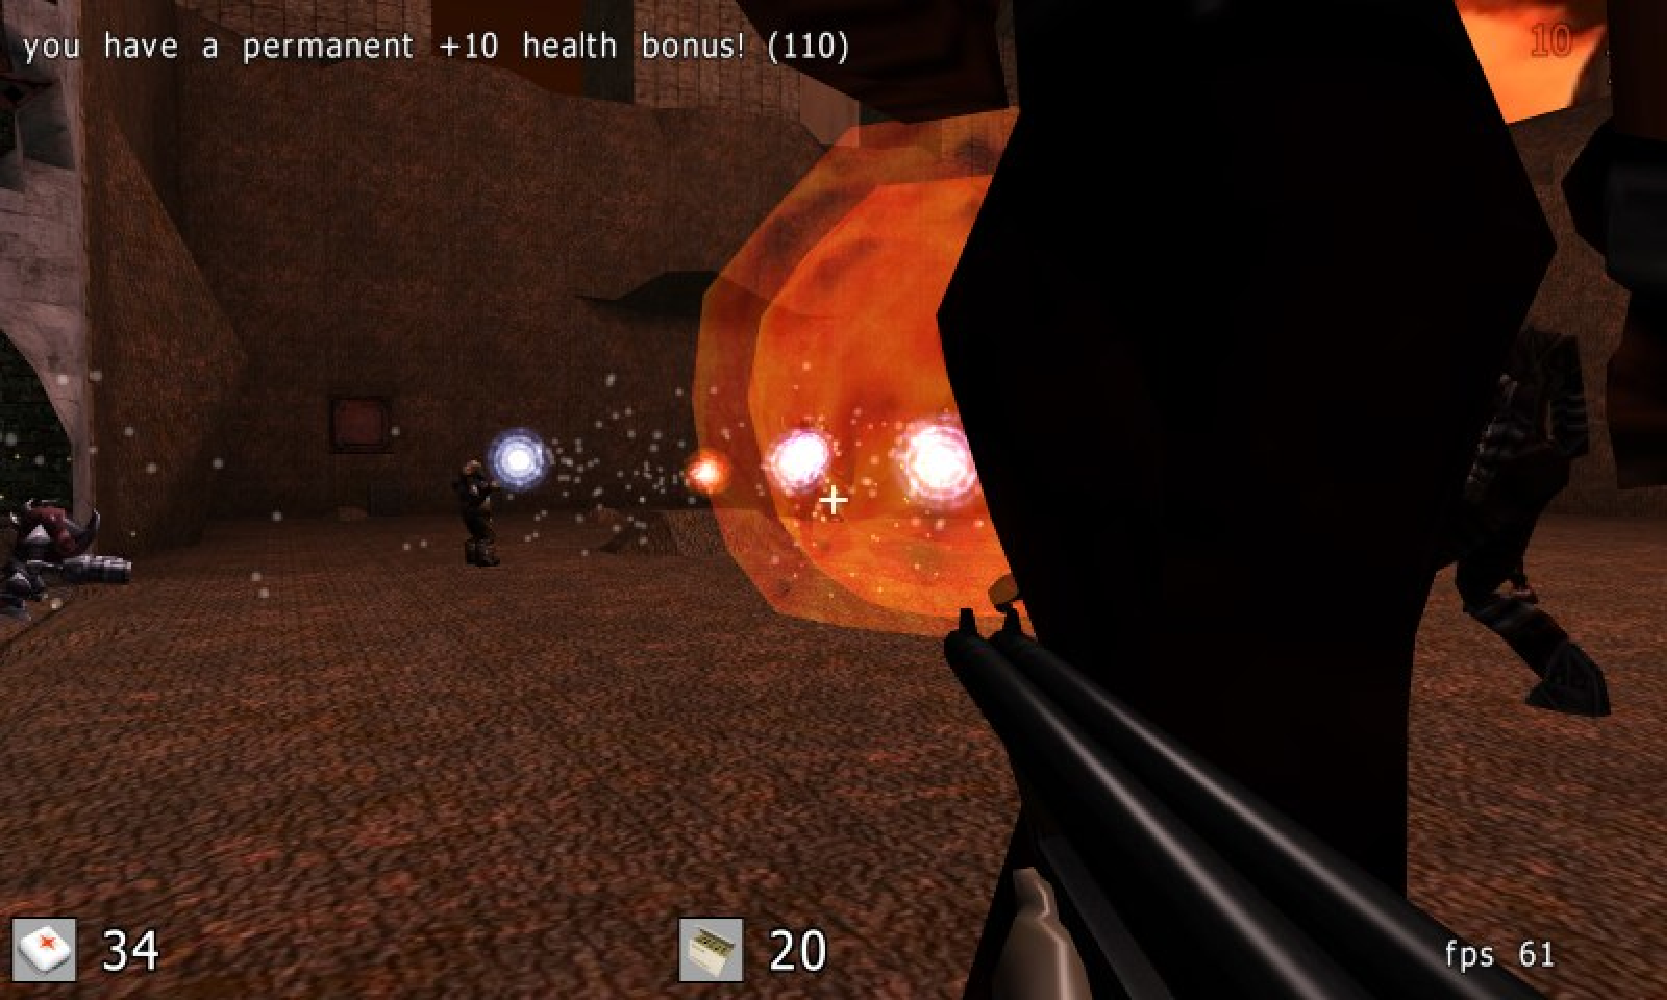
\includegraphics[width=10cm]{screenshot_5891783.pdf}\\
\href{http://sauerbraten.org/}{Capture d'écran de Cube 2}
        \end{center}
    \end{minipage}
    \hspace{1mm}
    \begin{minipage}{0.5\textwidth}
        \begin{center}
\input{Fig_VMNerGf.pstricks}
        \end{center}
    \end{minipage}

    Les joueurs \( A\) et \( B\) sont dans la situation ci-dessus et tirent dans les directions indiquées par les vecteurs dessinés. Vont-ils survivre ? 
    
\corrref{smath-0339}
\end{exercice}
